
\documentclass[a4paper,10pt]{report}

%\usepackage[landscape]{geometry}
\usepackage[cm-default]{fontspec}
\setromanfont{FreeSerif}
\setsansfont{FreeSans}
\setmonofont{FreeMono}
\usepackage[utf8x]{inputenc}
\usepackage{fontspec}
\usepackage{xunicode}
\usepackage{xltxtra}
\usepackage{xgreek}
\usepackage{amsmath}
\usepackage{unicode-math}
\usepackage{ulem}
\usepackage{color}
\usepackage{verbatim}
\usepackage{nopageno}
\usepackage{graphicx}
\usepackage{textpos}
\setlength{\TPHorizModule}{1cm}
\setlength{\TPVertModule}{1cm}
%\usepackage[colorgrid,texcoord]{eso-pic}
\usepackage[outline]{contour}
\usepackage{wrapfig}
\usepackage{url}
\usepackage{color}
\usepackage{tikz}
\usepackage{fancybox,fancyhdr}
\usepackage{subfigure}
\usepackage{pstricks}
\usepackage{epsfig}
\usepackage{multicol}
\usepackage{listings}
\usepackage{enumerate}
\usepackage{hyperref}
\hypersetup{
  bookmarks=true,
  bookmarksopen=true,
  pdfborder=false,
  pdfpagemode=UseNone,
  raiselinks=true,
  pdfhighlight={/P},
  colorlinks,
  citecolor=black,
  filecolor=black,
  linkcolor=black,
  urlcolor=black
}


\usepackage{fontspec}
\usepackage{xunicode}
\usepackage{xltxtra}


% Margins
%\setlength{\textwidth}{24cm}

%\setlength{\voffset}{0in}
%\setlength{\textheight}{6.8in}
% Colors
\definecolor{cbrown}{rgb}{0.49,0.24,0.07}
\definecolor{cmpez}{rgb}{0.92,0.88,0.79}
\definecolor{cmpez2}{rgb}{0.62,0.33,0.34}
\definecolor{cwhite}{rgb}{1,1,1}
\definecolor{cblack}{rgb}{0,0,0}
\definecolor{cred}{rgb}{0.9,0.15,0.15}
\definecolor{clblue}{rgb}{0.57,0.85,0.97}
\definecolor{corange}{rgb}{0.86,0.49,0.18}
\definecolor{clorange}{rgb}{0.95,0.84,0.61}
\definecolor{cyellow}{rgb}{1,0.95,0.16}
\definecolor{cgreen}{rgb}{0.69,0.8,0.31}
\definecolor{clbrown}{rgb}{0.78,0.67,0.43}
\definecolor{cmagenta}{rgb}{0.79,0.05,0.54}
\definecolor{cgray}{rgb}{0.76,0.73,0.63}
\definecolor{bluesite}{rgb}{0.05,0.43,0.67}
\definecolor{redsite}{rgb}{0.90,0.15,0.15}
\definecolor{backsite}{rgb}{0.07,0.07,0.07}
% ----------- from Costas -----------------------------

%---------------   Main Fonts    -----------------%   

% \setmainfont[Mapping=tex-text]{Calibri}
% \setmainfont[Mapping=tex-text]{Times New Roman}
%\setmainfont[Mapping=tex-text]{Droid Serif}
%\setmainfont[Mapping=tex-text]{Cambria}
%\setmainfont[Mapping=tex-text]{cm-unicode}
% \setmainfont[Mapping=tex-text]{Gentium}
% \setmainfont[Mapping=tex-text]{GFS Didot}
% \setmainfont[Mapping=tex-text]{Comic Sans MS}
 \setmainfont[Mapping=tex-text]{Ubuntu}
% \setmainfont[Mapping=tex-text]{Myriad Pro}
% \setmainfont[Mapping=tex-text]{CMU Concrete}
%\setmainfont[Mapping=tex-text]{DejaVu Sans}
%\setmainfont[Mapping=tex-text]{KerkisSans}
%\setmainfont[Mapping=tex-text]{KerkisCaligraphic}
% \setmainfont[Mapping=tex-text]{Segoe Print}
% \setmainfont[Mapping=tex-text]{Gabriola}

%------------------------------------------------%

% ------------ Mathematics Fonts ----------------%
\setmathfont{Asana-Math.ttf}
% -----------------------------------------------%
% Misc
\author{Κασωτάκη Ε. - Σμαραγδάκης Κ.}
\title{www.math24.gr}
% ---------------- Formation --------------------%


\setlength\topmargin{-0.7cm}
\addtolength\topmargin{-\headheight}
\addtolength\topmargin{-\headsep}
\setlength\textheight{26cm}
\setlength\oddsidemargin{-0.54cm}
\setlength\evensidemargin{-0.54cm}
%\setlength\marginparwidth{1.5in}
\setlength\textwidth{17cm}

\RequirePackage[avantgarde]{quotchap}
\renewcommand\chapterheadstartvskip{\vspace*{0\baselineskip}}
\RequirePackage[calcwidth]{titlesec}
\titleformat{\section}[hang]{\bfseries}
{\Large\thesection}{12pt}{\Large}[{\titlerule[0.9pt]}]
%--------------------------------------------------%
\usepackage{draftwatermark}
\SetWatermarkText{www.math24.gr}
\SetWatermarkLightness{0.9}
\SetWatermarkScale{0.6}
%--------------------------------------------------%


\usepackage{xcolor}
\usepackage{amsthm}
\usepackage{framed}
\usepackage{parskip}

\colorlet{shadecolor}{bluesite!20}

\newtheorem*{orismos}{Ορισμός}

\newenvironment{notation}
  {\begin{shaded}\begin{theorem}}
  {\end{theorem}\end{shaded}}




% Document begins
\begin{document}
\pagestyle{fancy}
\fancyhead{}
\fancyfoot{}
\renewcommand{\headrulewidth}{0pt}
\renewcommand{\footrulewidth}{0pt}


\fancyhead[LO,LE]{
 %\textblockcolor{backsite}
 %\begin{textblock}{5}(-2,-0.55)
  %\rule{0cm}{1cm}
 %\end{textblock}
 \textblockcolor{bluesite}
 \begin{textblock}{5}(-1.5,-0.55)
  \rule{0cm}{1cm}
 \end{textblock}
 %\textblockcolor{bluesite}
 %\begin{textblock}{14}(5.5,-0.55)
 % \rule{0cm}{1cm}
 %\end{textblock}
 \begin{textblock}{0}(-1,-0.25)
 \color{cwhite} \begin{Large}www.math24.gr\end{Large}
 \end{textblock}
\begin{textblock}{0}(16,-0.4)
 \color{cwhite} 
\includegraphics[height=1.5cm]{math24_logo.png}
 \end{textblock}
\textblockcolor{white}
\begin{textblock}{17}(-1,28)
 \color{backsite} \begin{small}Copyright \textcopyright 2011, Κασωτάκη Ε.(ikasotaki@gmail.com) - Σμαραγδάκης Κ.(kesmarag@gmail.com)\end{small}
 \end{textblock}
}
 
\begin{shaded}
\begin{center}
\huge \textbf{Φυλλάδιο Ασκήσεων}\\
%Πρόσθεση ρητών αριθμών
\end{center} 
\textbf{Μαθηματικά Α' Γυμνασίου} \hfill \textbf{Ημερομηνία Παράδοσης : \hspace{2em} }
\subsection*{Ονοματεπώνυμο :\hfill  \hspace{5em}}
\end{shaded}
\vspace{2em}
\begin{itemize}
 \item Τοποθέτηση στην ευθεία των αριθμών ενός κλάσματος που είναι μικρότερο της μονάδας
 \item Τοποθέτηση στην ευθεία των αριθμών ενός κλάσματος που είναι μεγαλύτερο της μονάδας
\end{itemize}



\section*{Θεωρία\\Τοποθέτηση στην ευθεία των αριθμών του κλάσματος $\dfrac{μ}{ν}$, με $μ<ν$ \hfill \small{}}
Για να τοποθετήσουμε στην ευθεία των αριθμών ένα κλάσμα που είναι μικρότερο από τη μονάδα, δηλαδή 
ένα κλάσμα της μορφής $\dfrac{μ}{ν}$ με $μ<ν$ εκτελούμε τα παρακάτω βήματα:
\begin{itemize}
 \item \textbf{1ο Βήμα:} Υπολογίζουμε ανάμεσα σε ποιους φυσικούς αριθμούς βρίσκεται το κλάσμα.
 \item \textbf{2ο Βήμα:} Χωρίζουμε την απόσταση των φυσικών αριθμών, στην οποία βρίσκεται το κλάσμα, 
              σε $ν$ ίσα μέρη (επειδή ο παρονομαστής είναι $ν$).
 \item \textbf{3ο Βήμα:} Το κλάσμα $\dfrac{μ}{ν}$ τοποθετείται στο σημείο εκείνο που απέχει 
               από το Ο απόσταση ίση με $μ\cdot \dfrac{1}{ν}$ της απόστασης των φυσικών αριθμών
               στους οποίου ανάμεσα (είχαμε υπολογίσει ότι) βρίσκεται το κλάσμα $\dfrac{μ}{ν}$. 
\end{itemize}

\textbf{Παράδειγμα} \\
Θέλουμε να τοποθετήσουμε στην ευθεία των αριθμών το κλάσμα $\dfrac{3}{4}$
\begin{itemize}
\item \textbf{1ο Βήμα:} Γνωρίζουμε ότι $0<\dfrac{3}{4}<\dfrac{4}{4}=1$. Δηλαδή το $\dfrac{3}{4}$ βρίσκεται 
      μεταξύ των φυσικών αριθμών $0$ και $1$.
 \item \textbf{2ο Βήμα:} Χωρίζουμε το $ΟΑ$ σε 4 ίσα μέρη (επειδή ο παρονομαστής του κλάσματος ισούται με 4).
 \item \textbf{3ο Βήμα:} Το κλάσμα $\dfrac{3}{4}$ τοποθετείται στο σημείο $Β$ επειδή το σημείο $Β$ απέχει 
       από το $Ο$ απόσταση ίση με τα $\dfrac{3}{4}$ του $ΟΑ$ 
\end{itemize}

\begin{figure}[ht]
\centering
\label{apotelesmata_sel14}
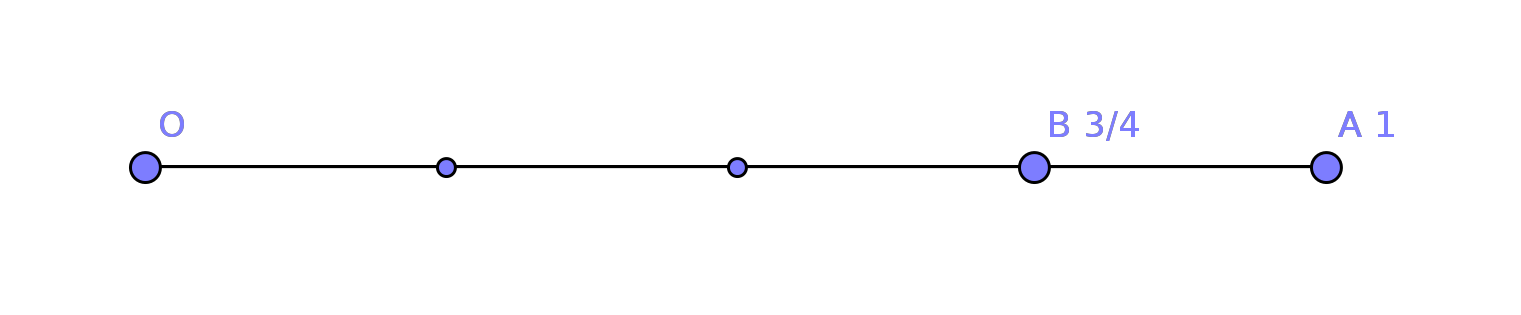
\includegraphics[scale=1]{theoria1.png}
%\caption{\textit{Σύνολο Αποτελεσμάτων}}
\end{figure}

\section*{Άσκηση 1  \hfill \small{25 μονάδες}}
Να τοποθετήσετε στην ευθεία των αριθμών το κλάσμα $\dfrac{3}{4}$.

\section*{Άσκηση 2  \hfill \small{25 μονάδες}}
Να τοποθετήσετε στην ευθεία των αριθμών το κλάσμα $\dfrac{5}{6}$.


\section*{Θεωρία\\Τοποθέτηση στην ευθεία των αριθμών του κλάσματος $\dfrac{μ}{ν}$, με $μ>ν$ \hfill \small{}}
Για να τοποθετήσουμε στην ευθεία των αριθμών ένα κλάσμα που είναι που είναι μεγαλύτερο από τη μονάδα, δηλαδή 
ένα κλάσμα της μορφής $\dfrac{μ}{ν}$ με $μ>ν$ εκτελούμε τα παρακάτω βήματα:
\begin{itemize}
 \item \textbf{1ο Βήμα:} Υπολογίζουμε ανάμεσα σε ποιους φυσικούς αριθμούς βρίσκεται το κλάσμα.
 \item \textbf{2ο Βήμα:} Χωρίζουμε τις αποστάσεις μεταξύ κάθε δύο φυσικών αριθμών 
              σε $ν$ ίσα μέρη επειδή ο παρονομαστής είναι $ν$ (δηλαδή χωρίζουμε την απόσταση 
              από το $0$ μέχρι το $1$ σε $ν$ ίσα μέρη, την απόσταση 
              από το $1$ μέχρι το $2$ σε $ν$ ίσα μέρη κ.τ.λ μέχρι και την απόσταση των φυσικών αριθμών 
              ανάμεσα στους οποίους βρίσκεται το κλάσμα.
 \item \textbf{3ο Βήμα:} Το κλάσμα $\dfrac{μ}{ν}$ τοποθετείται στο σημείο εκείνο που απέχει 
               από το Ο απόσταση ίση με $μ\cdot \dfrac{1}{ν}$. 
\end{itemize}

\textbf{Παράδειγμα} \\
Θέλουμε να τοποθετήσουμε στην ευθεία των αριθμών το κλάσμα $\dfrac{5}{3}$
\begin{itemize}
\item \textbf{1ο Βήμα:} Γνωρίζουμε ότι $1=\dfrac{3}{3}<\dfrac{5}{3<\dfrac{6}{3}}=2$.
      Άρα  το κλάσμα $\dfrac{5}{3}$ βρίσκεται 
      μεταξύ των φυσικών αριθμών $1$ και $2$.
 \item \textbf{2ο Βήμα:} Χωρίζουμε το $ΟΑ$ και το $ΑΒ$ σε 3 ίσα μέρη το καθένα 
 (επειδή ο παρονομαστής του κλάσματος ισούται με 3).
 \item \textbf{3ο Βήμα:} Το κλάσμα $\dfrac{5}{3}$ τοποθετείται στο σημείο $Γ$ επειδή το σημείο $ΟΓ$ αποτελείται 
        από 5 ίσα τμήματα ίσα με $\dfrac{1}{3}$ της μονάδας το καθένα.
       από το $Ο$ απόσταση ίση με τα $\dfrac{3}{4}$ του $ΟΑ$ 
\end{itemize}

\begin{figure}[ht]
\centering
\label{apotelesmata_sel14}
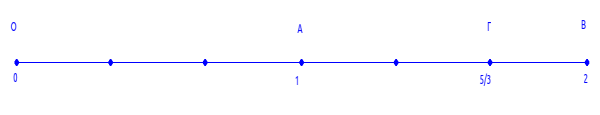
\includegraphics[scale=1]{theoria1b.png}
%\caption{\textit{Σύνολο Αποτελεσμάτων}}
\end{figure}


\section*{Άσκηση 3  \hfill \small{25 μονάδες}}
Να τοποθετήσετε στην ευθεία των αριθμών το κλάσμα $\dfrac{7}{4}$.
\section*{Άσκηση 4  \hfill \small{25 μονάδες}}
Να τοποθετήσετε στην ευθεία των αριθμών το κλάσμα $\dfrac{11}{5}$.








\end{document}
